% !Mode:: "TeX:UTF-8"
% !TEX program  = xelatex
\section{电气系统}

\subsection{引言}

电气系统包括供电、通讯、控制、传感等在内的所有电子元器件和由之组成的网络结构。轮腿机器人拥有若干对供电需求不一的电子元器件,也具有层级关系的通讯与控制网络,还需要能接受遥控器的控制,并将自身的状态回传。此外,后期可能安装在轮腿机器人上的其他电气部件也需要纳入考虑范围。在本章中,引言将会大致介绍上述的网络逻辑图,然后在每个子章节介绍重要的部件。电气系统示意图如图\ref{fig:sec3-sys}所示。

\begin{figure}[h!]
  \centering
  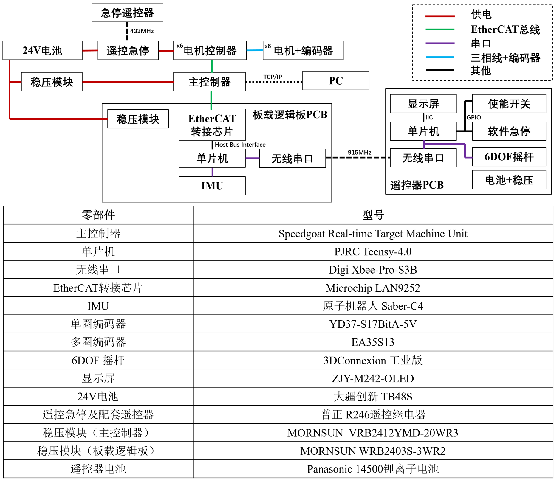
\includegraphics[width=0.9\linewidth]{figures/Sec3/sys.png}
  \caption{
  上:电气系统示意图。下:示意图中关键零部件具体型号。
  }
  \label{fig:sec3-sys}
   \vspace{6pt}
\end{figure}

供电方面,电池将直接通过稳压模块为SpeedGoat主控制器供电,以即使在使用遥控急停的情况下也不会丢失数据;板载逻辑板的稳压模块与上述供电并联;然后遥控急停开关通过分电板直接连接电机控制器,遥控急停受一个单独的遥控器控制,可以切断所有电机的电源。

\begin{figure}[h!]
  \centering
  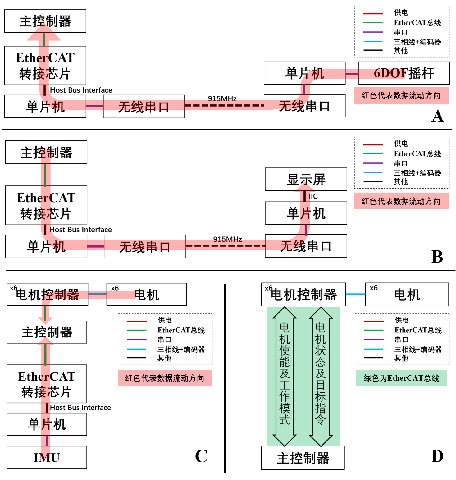
\includegraphics[width=0.9\linewidth]{figures/Sec3/comm.png}
  \caption{
  图A:运动控制指令由遥控器发送至主控制器处理。图B:机器人重要状态由主控制器发送至遥控器屏幕监看。图C:电机控制器、IMU反馈当前机器人状态给主控制器。图D:架设在电机控制器与主控制器间EtherCAT通讯网络上的两条虚拟通讯网络,分别是主控制器使能电机并决定电机工作状态,与主控制器发送电机与工作状态相应的运动指令。
  }
  \label{fig:sec3-comm}
   \vspace{6pt}
\end{figure}

通讯方面,最高层的通讯使用EtherCAT总线,使用菊花链的接线方式连接板载逻辑板、电机控制器和SpeedGoat主控制器。此外也可以使用TCP/IP与PC上位机的MATLAB Simulation进行通讯,实现程序下载、运行数据监看和参数调整等。板载逻辑板上的Teensy单片机会将EtherCAT总线中必要的数据,如电机的工作模式、电流等信息通过Xbee发送到遥控器以实现数据监看,遥控器也会回传运动指令。此外,遥控器可以远程静能所有电机,实现软件层面的另一种急停。IMU输出也是由该单片机将串口信号转换成EtherCAT信号。在这里,板载逻辑板内部的通讯构架是串口与Xbee提供的无线串口抽象。电机与电机控制器的通讯与控制是同时进行的:电机的转子位置信息通过编码器传输给电机控制器,而电机控制器直接传输驱动电流。

在EtherCAT通讯总线上,虚拟抽象出了以下两种数据链路:其一是用于决定电机使能静能、工作状态的底层控制数据链路;其二则是电机的转子位置、转子速度、转子加速度,和IMU的姿态、6轴加速度、6轴速度,作为系统的反馈提供给观测器,以获取状态变量。

\subsection{驱动模块}

驱动模块对于轮腿机器人而言至关重要,不但轮腿机器人的运动完全来自于驱动模块,而且驱动模块决定了机器人整体的性能。驱动模块包括电机本身、减速器、电机控制器和编码器等传感器。在上一章中,电机及其用途、机械性能已经被展示了,且准直驱电机包括了电机本身与减速器,因此下文所指的电机将包括减速器。在这里,更详细的电机的尺寸与电气参数如图\ref{fig:sec3-motors}所示。

\begin{figure}
  \centering
  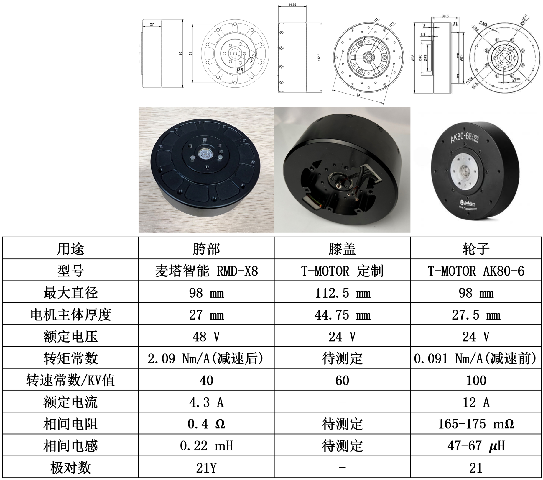
\includegraphics[width=0.85\linewidth]{figures/Sec3/motors.png}
  \caption{
  上图:电机尺寸。下图:尺寸及电气参数。
  }
  \label{fig:sec3-motors}
   \vspace{6pt}
\end{figure}

如上文所述,电机控制器通过编码器的位置反馈控制电机,且可以工作在包括位置模式、速度模式、电流模式等若干个模式。而在使用之前,需要但对每个电机进行三环调试。虽然轮腿工作在力控模式下时,无需调试速度和位置模式,但这些模式对初始化与实验调试必不可少。
准直驱的力控模式的实现原理是,根据电流和电动机的扭矩常数、减速比,计算出输出扭矩,也可以根据期望扭矩计算出目标电流。而扭矩常数往往有偏差或电机本身线性程度不好,需要对电机进行标定并选取工作范围内的数据,重新计算扭矩常数。
如引言所述,对于SpeedGoat中抽象的控制程序,电机的状态反馈必不可少,而电机控制器会根据编码器位置信息,计算出上述需求的反馈量。

\subsubsection{电机三环调试}
三环调试是指上一节所说的位置模式、速度模式和电流模式。其中电流模式是在输入和标定电机参数之后,通过伺服控制器内建的控制器实现电流环。在此基础上,通过PI控制器是实现速度环,而控制器的参数则是需要根据电机跟踪效果调节的。再在速度环的基础上,通过P控制器实现位置环,同样P参数也需要通过电机跟踪效果调节。调试过后这些参数保存在控制器中。

\subsubsection{电流-扭矩关系标定}
电机的扭矩在一定范围内与电流有很强的线性关系,虽然扭矩常数随电机转速会发生变化,但考虑到轮腿的工况,简化起见,仅标定静止状态下的电机扭矩常数。由于目前膝盖、胯部电机主要工作在位置模式,所以本毕设仅标定了轮子电机,但实际上电机的标定过程是相同的。如图\ref{fig:sec3-tauIplot}所示,标定的方式是,给定斜坡电流信号,然后通过力传感器读出已知距离处产生的力,便可根据力臂计算出扭矩。在获取原始的扭矩-电流信息后,选取实际工况所在范围,然后通过最小二乘的方式计算出斜率,从而计算出扭矩常数,如图\ref{fig:sec3-tauIplot}所示。

\begin{figure}
  \centering
  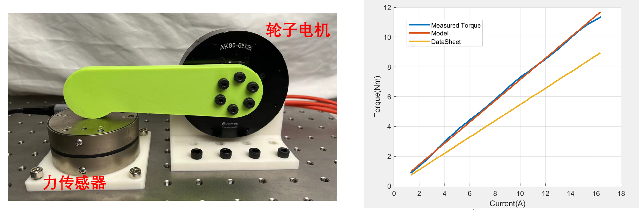
\includegraphics[width=0.85\linewidth]{figures/Sec3/tauIplot.png}
  \caption{
  左图:电机电流扭矩曲线测定实验平台。右图:电流扭矩实际曲线、根据最小二乘计算的曲线和厂商说明书给定的曲线。
  }
  \label{fig:sec3-tauIplot}
   \vspace{6pt}
\end{figure}

\subsubsection{电机控制器和编码器}
电机控制器和编码器的详细型号如图\ref{fig:sec3-escen}所示。电机控制器除了接受对应工作模式的指令、反馈电机的状态外,在进入这些模式之前,需要使能。与之相对应的,当电机驱动器静能之后,电机便不再输出扭矩。静能只需要将电机控制器的CMD WORD置为0,而出于安全考虑,使能过程较为复杂,以防止电机误使能发生意外。概括而言,电机驱动器会周期性发送STATUS WORD,主控制器需要连续若干次根据事先约定的计算方式根据STATUS WORD计算出正确的CMD WORD以使能电机,具体如图\ref{fig:sec3-motoren}所示。
使能后,电机驱动器通过OP MODE信息决定工作模式,会将与工作模式对应的指令作为目标状态,控制电机达到这些状态,而电机的工作状态,也就是上文提到的实际转子位置、速度、加速度、电流等等都以EtherCAT的通讯频率发送至主控制器。
关于编码器,值得注意的是,轮子编码器并需要绝对位置信息,而其他电机使用绝对位置编码器,具有断电后保存的功能,使得每次机器人初始化无需进行工作空间和电机行程的标定。但仍然必须进行工作空间和电机行程的标定,并作为配置文件记录在主控制器中。

\begin{figure}[h!]
  \centering
  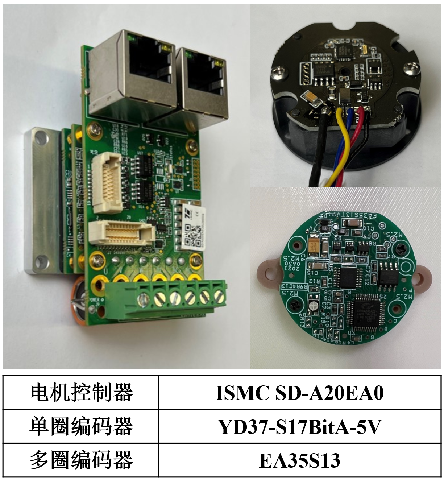
\includegraphics[width=0.6\linewidth]{figures/Sec3/escen.png}
  \caption{
  左图:电机控制器。右上图:单圈编码器,用与轮子电机。右下图:多圈编码器,用于膝盖、胯部的电机,需要外接电池,可以机器人关闭后保存位置信息,当机器人启动后,电池会自动充电;保存位置信息使得机器人免于每次上电时都需要校准膝盖和胯部的行程。
  }
  \label{fig:sec3-escen}
   \vspace{6pt}
\end{figure}

\begin{figure}
  \centering
  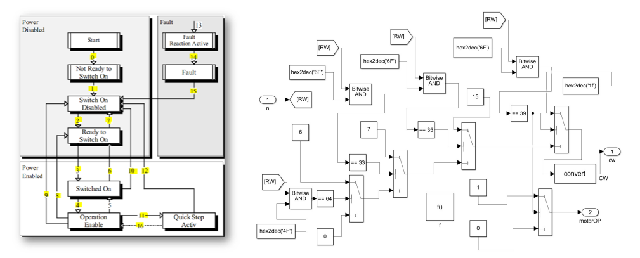
\includegraphics[width=0.85\linewidth]{figures/Sec3/motoren.png}
  \caption{
  左图:电机驱动器中关于电机使能方式的说明。右图:实际在Simulink中的使能程序截图。
  }
  \label{fig:sec3-motoren}
   \vspace{6pt}
\end{figure}

\subsection{SpeedGoat控制器}
SpeedGoat控制器是基于QNX操作系统的商业化实时工业控制器,其支持EtherCAT、CAN等通讯,使用MATLAB Simulink进行编程,相比于传统的基于Linux和ROS的PC作为控制器,具有敏捷开发、硬件实时、便于数据监看与记录、减少并行化程序错误的优点。本毕设采用的SpeedGoat控制器的如图\ref{fig:sec3-speedgoat}所示,其体积与功耗较小,但可实现EtherCAT总线1000Hz的通讯,且对EtherCAT通讯支持较好。使用MATLAB Simulink进行编程时,可以留出统一接口,方便将为MATLAB Simulink Simscapes仿真模型设计的控制器迁移到实物,或实现数字孪生功能。Simulink编程解决了并行化的大多数问题,如内存同时访问,资源上锁、调度等,且提供直观的数据监看和记录,并可以在MATLAB中进行快速处理。Simulink也可以调用MATLAB程序,并编译执行,以实现与编译型语言类似的执行速度;MATLAB则提供了丰富高效的线性代数、优化、学习、机器人运动控制等库,且编程简单快速。使用这种开发模式,可以实现一种类似于元编程(Meta-programming)的效果。

\begin{figure}
  \centering
  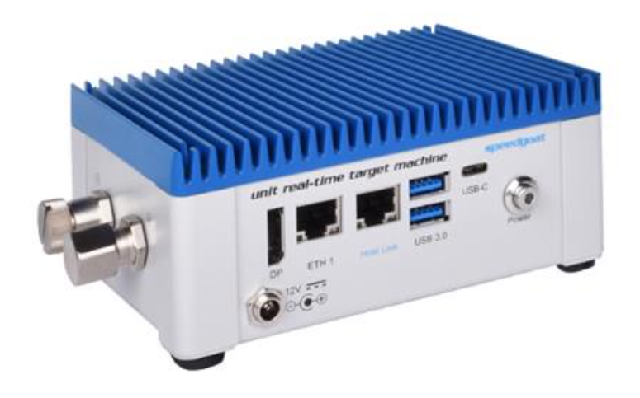
\includegraphics[width=0.6\linewidth]{figures/Sec3/speedgoat.png}
  \caption{
  Speedgoat Real Time Target Machine Unit示意图。
  }
  \label{fig:sec3-speedgoat}
   \vspace{6pt}
\end{figure}

\subsection{板载逻辑板等部件}
如引言所述,板载逻辑板包括了稳压模块,Teensy 4.0 单片机,EtherCAT转接芯片,IMU和Xbee。其具体如图\ref{fig:sec3-logicbd}所示。其中稳压模块负责供电,而Teensy单片机负责将数据从Xbee传入和传出EtherCAT总线,并将IMU数据转换至EtherCAT总线。
Teensy单片机支持开源Arduino社区的库,并可以使用与Arduino相同的方式编程,但其芯片采用ARM Cortex-M7内核,核心频率高达600MHz,且可以超频的超线程处理;其拥有丰富的外设和GPIO,并且CPU具有缓存及分支预测设计,并支持32位浮点数和DSP指令。其体积小巧,开发快速。
Xbee是Digi公司根据ZigBee协议设计的多功能无线串口。其延迟约为数十毫秒,体积小,功耗低,但连接稳定,调试方便,带宽大。Teensy单片机会从EtherCAT总线读取电机和IMU的状态,然后通过Xbee发送至遥控器及数据监看;而遥控器会给出运动指令,并兼具初始化电机使能和软件急停的功能,这些信息也都通过Teensy从Xbee读出后发送至EtherCAT总线,然后通过SpeedGoat主控制实现。Teensy单片机完全负责通讯转换的工作。

\begin{figure}
  \centering
  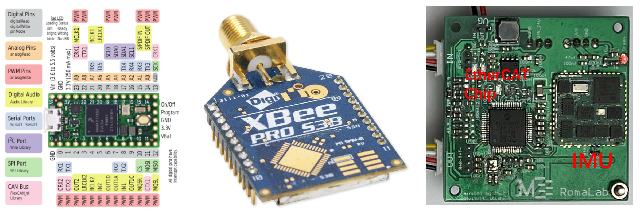
\includegraphics[width=0.85\linewidth]{figures/Sec3/logicbd.png}
  \caption{
  左图:Teensy单片机。中图:Xbee模块。右图:IMU及EtherCAT转接芯片。
  }
  \label{fig:sec3-logicbd}
   \vspace{6pt}
\end{figure}

\subsection{遥控及数据监看}

\begin{figure}[h!]
  \centering
  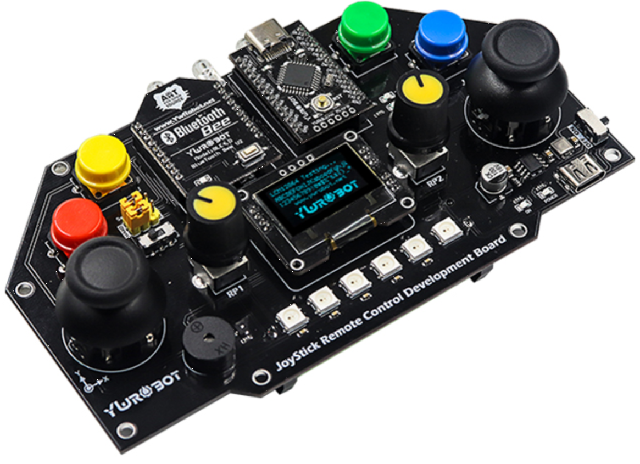
\includegraphics[width=0.75\linewidth]{figures/Sec3/rmctrl.png}
  \caption{
  遥控器示意图
  }
  \label{fig:sec3-rmctrl}
   \vspace{6pt}
\end{figure}

考虑到市面上成熟的RC遥控器多使用PPM或者Sbus通讯协议,并仅支持少数简单传感器信号回传,而轮腿机器人回传信息较为复杂。且这些遥控器虽然控制模型飞机,但其使用两个XY摇杆控制,仅能控制4自由度运动,操作并不直观。因此本毕设自主设计了遥控器,其系统图如图\ref{fig:sec3-rmctrl}。

其中3Dconnexion摇杆具有6个自由度,虽然轮腿仅能实现至多4个自由度的单独控制,但该摇杆非常直观,与运动指令一一对应,而无需考虑XY摇杆的映射问题。Xbee负则实现无线通讯,Teensy单片机则将机器人回传的信息通过串口读出,并通过OLED屏幕或RGB指示灯显示。而机器人的电机使能和静能,软件急停和上述运动控制指令也通过Xbee发送到机器人。

\subsection{本章小结}

本章介绍了电气系统。首先介绍了电气系统的整体框图,包括EtherCAT总线及挂载在总线上的各个设备,包括电机驱动器、主控制器和IMU,并逐一介绍他们。在介绍电机驱动器时,同时介绍了编码器、电机的三环调试和电流、扭矩曲线标定。在介绍IMU的部分,同时介绍了遥控通讯系统和遥控器的设计及数据监看。
